\section{Konstruktionen mit Zirkel und Lineal}
Sei $M$ eine Menge von Punkten in der Ebene $\R^2 = \C$. Wir wollen auf $M$ mittels elementarer Konstruktionen neue Punkte erzeugen. 

\textbf{Elementare Konstruktionen:}
\begin{enumerate}[label=(\Roman*)]
	\item\label{konstr1} Schnitt zweier verschiedener Geraden durch Punkte in $M$ bilden.
	\item\label{konstr2} Schnitt zwei verschiedener Kreise mit Mittelpunkt in $M$ bilden, deren Radius der Abstand zweier Punkte in $M$ ist.
	\item\label{konstr3} Schnitt einer Geraden und eines Kreises bilden, die wie zuvor durch Punkte in $M$ gegeben sind. 
\end{enumerate}
Sei $\{0,1\} \subseteq M \subseteq \C$ und $\tilde{M} \subseteq \C$ die Menge der Punkte, die sich aus $M$ in endlich vielen Schritten mittles der Konstruktionen \ref{konstr1}, \ref{konstr2} und \ref{konstr3} konstruieren lassen.
\begin{satz}\label{satz9_1}
	$\tilde{M}$ ist ein Teilkörper von $\C$ und \textbf{quadratisch abgeschlossen}, d. h. für $z \in \C$ mit $z^2 \in \tilde{M}$ folgt $z \in \tilde{M}$.
\end{satz}
\begin{proof}
	\underline{Addition:} Seien $u, v \in \tilde{M}$. Sind $u$ und $v$ $\R$-linear abhängig, so ist $u + v$ Schnittpunkt des Kreises um $u$ mit Radius $|v-0|$ und der Geraden durch $0$ und $u$. Sind $u$ und $v$ $\R$-linear unabhängig, so ist $u+v$ Schnittpunkt der Kreise um $u$ mit Radius $|v-0|$ und um $v$ mit Radius $|u-0|$.
	
	\begin{center}
		\begin{tikzpicture}
			% Koordinatensystem
			\draw[->] (-1, 0) -- (5, 0) node[right] {};
			\draw[->] (0, -1/2) -- (0, 3) node[above] {};
			
			% Vektoren u und v
			\coordinate (O) at (0, 0); % Ursprung
			\coordinate (u) at (3, 1); % Vektor u
			\coordinate (v) at (-1, 2); % Vektor v
			\coordinate (uplusv) at ($(u) + (v)$); % Vektor u + v
			
			% Zeichne das Parallelogramm
			\draw[thick, -] (O) -- (u) node[midway, below] {};
			\draw[thick, -] (O) -- (v) node[midway, left] {};
			\draw[thick, -] (u) -- (uplusv) node[midway, right] {};
			\draw[thick, -] (v) -- (uplusv) node[midway, above] {};
			\draw[dashed] (u) -- (uplusv) (v) -- (uplusv);
			
			% Beschriftung für u + v am Punkt u + v
			\node at (uplusv) [above right] {$u + v$};
			\node at (u) [right] {$u$};
			\node at (v) [left] {$v$};
		\end{tikzpicture}
		
	\end{center}
	
	Ist $z \in \tilde{M} \setminus \{0\}$, so ist $-z$ Schnittpunkt der Geraden durch $0$ und $z$ und dem Kreis um $0$ mit Radius $|z-0|$
	
	\underline{Multiplikation:} Sei $u = re^{i\varphi}, v = se^{i\psi} \in \tilde{M} \setminus \{0\}$. Wir zeigen, dass $uv^{-1} = rs^{-1} e^{i(\varphi - \psi)} \in \tilde{M} \setminus \{0\}$. Es gilt $|u| = r, |v| = s \in \tilde{M}$, da wir entsprechende Kreise um $0$ mit der Geraden durch $0$ und $1$ schneiden können. Da sich mit Zirkel und Lineal Lote fällen bzw. errichten lassen, ist die folgende Figur konstruierbar:
	
	\begin{center}
		\begin{tikzpicture}
			% Koordinaten des Dreiecks
			\coordinate (A) at (0, 0);    % Punkt A (rechter Winkel)
			\coordinate (B) at (4, 0);    % Punkt B (rechts)
			\coordinate (C) at (4, 3);    % Punkt C (oben)
			
			% Zeichne das Dreieck
			\draw[thick] (A) -- (B) -- (C) -- cycle;
			
						
			% Beschriftungen der Seiten
			\node at ($(A)!0.5!(B)$) [below] {$s$};  % Seite a (unten)
			\node at ($(A)!0.5!(C)$) [left] {};   % Seite b (links)
			\node at ($(B)!0.5!(C)$) [above right] {$rs^{-1}$}; % Seite c (Hypotenuse)
			
			% Punkte beschriften (optional)
			\node at (A) [below left] {$0$};
			\node at (B) [below right] {$r$};
			\node at (C) [above left] {};
			
			\draw[thick] ($(A)!0.5!(B)$) -- ++(0, 1.5) node[midway, right] {$1$};
		\end{tikzpicture}
	\end{center}
	
	Somit gilt $rs^{-1} \in \tilde{M}$. 
	
	Wir erhalten $e^{i \varphi}, e^{i \psi} \in \tilde{M}$ als Schnitt der Geraden durch $0$ und $u$ bzw. $v$ mit dem Einheitskreis. Zudem ist $e^{i(\varphi - \psi)} \in \tilde{M}$ ein Schnittpunkt des Kreises um $e^{i\varphi}$ mit Radius $|e^{i\psi} - 1|$ und dem Einheitskreis.
	
	\begin{center}
		
		\begin{tikzpicture}[scale=3]
			
			\coordinate (O) at (0, 0); % Ursprung
			\coordinate (U) at (0.7, 1.5);    % Punkt A (rechter Winkel)
			\coordinate (V) at (1.5, 0.5);    % Punkt B (rechts)
			\coordinate (UV) at (1.1, -0.6);
			\coordinate (X) at (1,0);
			\coordinate (Y) at (0,1);
			
			% Koordinatensystem
			\draw[->] (-1.4, 0) -- (1.4, 0) node[right] {}; % x-Achse
			\draw[->] (0, -1.4) -- (0, 1.4) node[above] {}; % y-Achse
			
			% Einheitskreis
			\draw[thick] (0, 0) circle (1);
			
			
			\draw[thick, -] (O) -- (U) node[midway, below] {};
			\draw[thick, -] (O) -- (V) node[midway, below] {};
			\draw[thick, -] (O) -- (UV) node[midway, below] {};		
			
		
			\pic["\color{red}$\varphi - \psi$", draw=red, -, angle eccentricity=0.6, angle radius=3.2cm]
			{angle=UV--O--X};
			\pic["\color{red}$\psi$", draw=red, -, angle eccentricity=0.6, angle radius=3.8cm]
			{angle=X--O--U};
			
			\pic["\color{red}$\varphi$", draw=red, -, angle eccentricity=0.6, angle radius=3.5cm]
			{angle=X--O--V};
			
			\node at (U) [right] {$u$};
			\node at (V) [right] {$v$};
			\node at (UV) [right] {$uv^{-1}$};
		\end{tikzpicture}
	\end{center}
	\color{black}

	
	Die Gerade durch $0$ und $e^{i(\varphi - \psi)}$ schneidet den Ursprungskreis mit Radius $|rs^{-1} - 0|$ im Punkt $rs^{-1} e^{i(\varphi - \psi)}$, d. h. $uv^{-1} \in \tilde{M}$.
	
	\underline{Noch zu zeigen:} $u = re^{i \varphi} \in \tilde{M} \setminus \{0\} \;\Rightarrow\; \sqrt{r} e^{i\varphi / 2} \in \tilde{M}$.
	
	Da $r \in \tilde{M}$ und $\tilde{M}$ Körper ist, folgt $\frac{r-1}{2} \in \tilde{M}$. Wir konstruieren folgende Figur:
	
	\begin{center}
		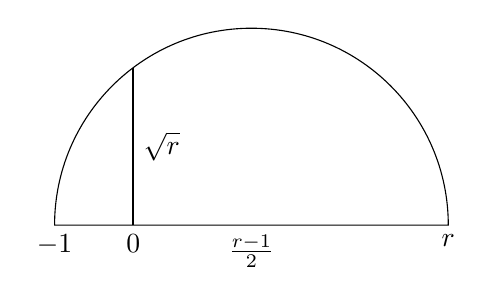
\begin{tikzpicture}[baseline=(current bounding box.north)]
			
			\coordinate (M) at (-2.5, 0); 
			\coordinate (O) at (-1.5, 0); 
			\coordinate (OS) at (-1.5, 2.0);
			\coordinate (R) at (2.5,0); 
			
			\coordinate (MID) at (0,0); 
			
			
			\draw (-2.5,0) -- (2.5,0) arc(0:180:2.5) --cycle;
			\draw[thick, -] (O) -- (OS) node[midway, right] {$\sqrt{r}$};
			
			\node at (M) [below] {$-1$};
			\node at (O) [below] {$0$};
			\node at (R) [below] {$r$};
			\node at (MID) [below] {$\frac{r-1}{2}$};
			
			%
			%%Labels for the vertices are typeset.
			
		\end{tikzpicture}
	\end{center}
	
	Also gilt $\sqrt{r} \in \tilde{M}$. Da Winkelhalbierende mit Zirkel und Lineal konstruierbar sind, ist auch $e^{i\varphi / 2} \in \tilde{M}$ und die Behauptung folgt.
\end{proof}
\begin{lem}\label{lem9_2}
	Sei $K \subseteq \C$ ein Teilkörper mit $i \in K$ und $K$ abgeschlossen unter komplexer Konjugation. Wird $\alpha$ aus $K$ mithilfe von einer Elementarkonstruktion erzeugt, so gilt $K(\alpha) :K] \leq 2$ und $K(\alpha)$ ist abgeschlossen unter Konjugation.
\end{lem}
\begin{proof}[Beweisidee]
	\begin{enumerate}[label=\arabic*.)]
		\item Nutze, dass für $z = a + bi \in K$ auch $a,b \in K$ gilt. Damit haben Geradengleichungen und Kreisgleichungen, definiert durch Punkte aus $K$, Koeffizienten in $K \cap \R$.
		\item Fallunterscheidung bzgl. Elementarkonstruktionen:
		
		\underline{$\alpha$ erzeugt durch \ref{konstr1}:}
		Schnittpunkt zweier Geraden mit Koeffizienten in $K \cap \R$ liegt wieder in $K$, d. h. $K = K(\alpha)$.
		
		\underline{$\alpha$ erzeugt durch \ref{konstr3}:} Erhalten durch Einsetzen eine quadratische Gleichung mit Koeffizienten in $K \cap \R$. Adjungiere eine Nullstelle $\beta$ des entsprechenden Polynoms.  Dann gilt $K(\alpha) = K(\beta)$.
		
		\underline{$\alpha$ erzeugt durch \ref{konstr2}:} Differenz der Kreisgleichung liefert Geradengleichung mit Koeffizienten in $K \cap \R$. Jetzt weiter wie im Fall zuvor.
	\end{enumerate}
\end{proof}
\begin{satz}\label{satz9_3}
	Sei $\{0,1\} \subseteq M \subseteq \C$. Ein Element $z \in \C$ ist genau dann aus $M$ konstruierbar, wenn eine endliche Kette von Körpererweiterungen
	\[\Q(M \cup \{\bar{w} \mid w \in M\}) =: K_0 \leq K_1 \leq \dots \leq K_r\]
	existiert, so dass $[K_i : K_{i-1}] \leq 2$ und $z \in K_r$.
\end{satz}
\begin{proof}
	\glqq$\Rightarrow$\grqq: Sei $z \in \tilde{M}$. Es ist $K_0$ ein Teilkörper von $\tilde{M}$ und $i \in \tilde{M}$ nach Satz \ref{satz9_1}. Setzen $K_1 := K_0[i]$. Da $z$ aus $K_1$ mittels endlich vieler Elementarkonstruktionen erzeugt wird, liefert Lemma \ref{lem9_2} die Behauptung.
	
	\glqq$\Leftarrow$\grqq: Zeige per Induktion, dass alle Elemente in $K_r$ konstruierbar sind. Es gilt $K_0 \leq \tilde{M}$. Angenommen, alle Elemente in $K_{i-1}$ sind konstruierbar. Sei $[K_i : K_{i-1}] = 2$. Dann gibt es ein $\alpha \in K_i$ mit $K_i = K_{i-1} (\alpha)$. Sei $\mu_\alpha = x^2 + px + q$ das Minimalpolynom von $\alpha$ über $K_{i-1}$. Nach Satz \ref{satz9_1} ist dann $\alpha \in \{-\frac{p}{2} \pm \sqrt{\frac{p^2}{4} - q}\}$ konstruierbar und es folgt $K_i \subseteq \tilde{M}$. 
\end{proof}
\begin{kor}\label{kor9_4}
	Jede aus $M = \{0,1\}$ konstruierbare Zahl $z \in \C$ ist algebraisch über $\Q$ mit $[\Q(z) : \Q] = 2^s$ für ein $s \in \N_0$.
\end{kor}
\begin{proof}
	Nutze Satz \ref{satz9_3} und die Gradformel.
\end{proof}
\begin{beispiel}\label{beispiel9_5}
	\begin{enumerate}[label=(\arabic*)]
		\item \textbf{Delisches Problem:} Gegeben Würfel mit Kantenlänge 1. Lässt sich mit Zirkel und Lineal ein Würfel mit doppelten Volumens konstruieren, d. h. lässt sich $M = \{0,1\}$ die Zahl $\sqrt[3]{2}$ konstruieren? Da $[\Q(\sqrt[3]{2}) : \Q] = 3$ (siehe Beispiel \ref{beispiel7_15}), ist dies nicht möglich nach Korollar \ref{kor9_4}.
		\item \textbf{Quadratur des Kreises:} Gegeben ein Kreis mit Radius 1. Lässt sich mit Zirkel und Lineal ein Quadrat gleichen Flächeninhalts konstruieren, d. h. lässt sich aus $M = \{0,1\}$ die Zahl $\sqrt{\pi}$ konstruieren? Da $\pi$ transzendent über $\Q$ und somit $[\Q(\pi) : \Q] = \infty$, ist auch dies nicht möglich nach Korollar \ref{kor9_4}.
	\end{enumerate}
\end{beispiel}